\chapter{Arhitektura i dizajn sustava}

\noindent \\Pri analizi projektnih zahtjeva i detaljnom razmatranju uloga dionika te njihovih interakcija unutar aplikacije, odlučili smo strukturirati naš sustav na tri ključne razine: razinu klijenta, razinu web aplikacije i razinu baze podataka. Unutar ove podjele, nužno je uključiti slojeve korisničkog sučelja, aplikacijske logike i pristupa podacima. Kao model arhitekture, odabrali smo višeslojnu strukturu sličnu MVC (Model-View-Controller) stilu. MVC je oblik arhitekture softvera koji organizira aplikaciju u tri komponente:

\begin{itemize}
	\item 	\textit{Model (poslovna logika i podaci)}
	\item 	\textit{View (korisničko sučelje)}
	\item 	\textit{Controller (upravljač, posrednik između Modela i Viewa)}
\end{itemize}
\noindent Razdvajanje logike, prezentacije i upravljanja omogućuje jednostavno održavanje i razvoj aplikacije, a promjene u jednoj komponenti ne bi trebale značajno utjecati na druge. Ova arhitektura, bazirana na klijent-poslužitelj odnosu, omogućuje jasno definiranu organizaciju slojeva, a s ciljem maksimalne ponovne uporabivosti, integrirali smo i različite programske biblioteke i radne okvire. Razvojni tim je pisao kod u razvojnom okruženju IntelliJ IDEA i Visual Studio Code, a za pokretanje, konfiguraciju i puštanje u pogon, kao i neovisnost o računalu na kojem se kod izvršava, odabrali smo platforme Docker, Render i Node.JS.


\noindent \\Arhitektura web aplikacije "CestaFix" može se podijeliti na tri podsustava:
\begin{itemize}
	\item 	\textit{Web poslužitelj}
	\item   \textit{Web aplikacija}
	\item   \textit{Baza podataka}
\end{itemize}

\noindent\textbf{Web poslužitelj} je komponenta koja pruža podršku za backend sustav aplikacije i čija je ključna uloga omogućiti komunikaciju između klijenta i aplikacije. Ova interakcija odvija se putem HTTP (Hyper Text Transfer Protocol) protokola, standardnog protokola za prijenos informacija na webu. Pokretanje web aplikacije i prosljeđivanje zahtjeva aplikaciji radi daljnje obrade, inicira se upravo pomoću web poslužitelja. Za implementaciju web poslužitelja korišten je Spring Boot, Java framework, koji se ističe brzim konfiguriranjem i implementacijom web aplikacija temeljenih na Javi. Sastavljen od Model i Controller slojeva prema MVC arhitekturi, gdje se poslovna logika, kao što je upravljanje prijavama šteta, nalazi u Modelu. Web poslužitelj također omogućuje definiranje i implementaciju RESTful API-ja, što omogućuje komunikaciju između frontenda (klijenta) i backenda (poslužitelja) putem HTTP/HTTPS mrežnih protokola. Primarni zadatak Controllera unutar web poslužitelja je obrađivanje HTTP zahtjeva koji pristižu iz frontend dijela aplikacije, izvršavanje odgovarajuće funkcionalnosti te slanje odgovora. Dodatno, Spring Boot omogućuje učinkovito upravljanje stanjem aplikacije, uključujući praćenje stanja sesija za registrirane korisnike.
\newline
\textbf{\\Web preglednik} je softver koji djeluje kao posrednik između poslužitelja i klijenta, omogućujući korisniku prikaz web sadržaja. Osnovna funkcionalnost web preglednika ostvarena je pri slanju HTTP zahtjeva poslužitelju te prijemu i interpretaciji HTTP odgovora. Web preglednici djeluju kao prevoditelji, omogućavajući korisnicima vizualizaciju web sadržaja kroz sučelje preglednika, dekodiranjem informacija dobivenih iz HTTP odgovora.
\newline
\textbf{\\Web aplikacija} Web aplikacija je kompleksni softverski sustav koji se sastoji od frontend i backend dijelova:
\begin{itemize}
	\item \textbf{Frontend} (Klijent) predstavlja korisničko sučelje putem kojeg korisnici ostvaruju interakciju sa sustavom. Ostvaren je korištenjem JavaScript programskog jezika, za potrebu upravljanja događajima na korisničkom sučelju, i React radnog okvira, što omogućuje kreiranje dinamičnog i intuitivnog korisničkog sučelja, čime se ostvaruje ugodno korisničko iskustvo. Frontend je strukturiran u komponente, što olakšava održavanje i ponovnu uporabu koda. Komunicira s backendom kroz HTTPS zahtjeve te pritom omogućuje prijenos podataka i ažuriranje informacija o prijavama šteta. Kroz klijentsku logiku, frontend provodi validaciju unesenih podataka kako bi osigurao ispravnost prije slanja na backend. Responsivni dizajn osigurava konzistentno korisničko iskustvo na različitim uređajima.
	\item \textbf{Backend} (Poslužitelj) je dio sustava unutar kojeg se obrađuju zahtjevi i izvršavaju daljnje radnje. Kako bi se postiglo "razdvajanje zabrinutosti", organiziran je na kontrolere, servise i repozitorije. Controlleri imaju ključnu ulogu u obradi ulaznih zahtjeva (HTTP zahtjeva) omogučujući organizaciju i upravljanje tijekom rukovanja zahtjevima u backend dijelu aplikacije kao i pozivanje odgovarajućih metoda u Modelu te slanje odgovora klijentskom dijelu. Servisi u backendu na učinkovit i organiziran način obavljaju poslovnu logiku i specifične funkcionalnosti koje su potrebne za obradu zahtjeva, koji dolaze s frontend dijela aplikacije. Repozitoriji imaju ključnu ulogu u komunikaciji s bazom podataka, odnosno omogućuju servisima da abstrahiraju detalje interakcije s bazom podataka, pružajući im jednostavan i konzistentan način komunikacije s podacima. Backend je ostvaren korištenjem Java programskog jezika i Spring Boot radnog okvira. Također, pruža RESTful API-je koji omogućuju komunikaciju između klijenta i servera te definiraju kako resursi (poput prijava šteta) mogu biti stvoreni, ažurirani i dohvaćeni. Osim toga backend sadrži i DTO-e (Data Transfer Objects) za prijenos podataka između različitih dijelova sustava odnosno slojeva aplikacije.
\end{itemize}

\noindent \textbf{Baza podataka} je podatkovni sloj koji se koristi za sigurnu pohranu podataka te je detaljnije opisana u sljedećem poglavlju.

\begin{figure}[H]
	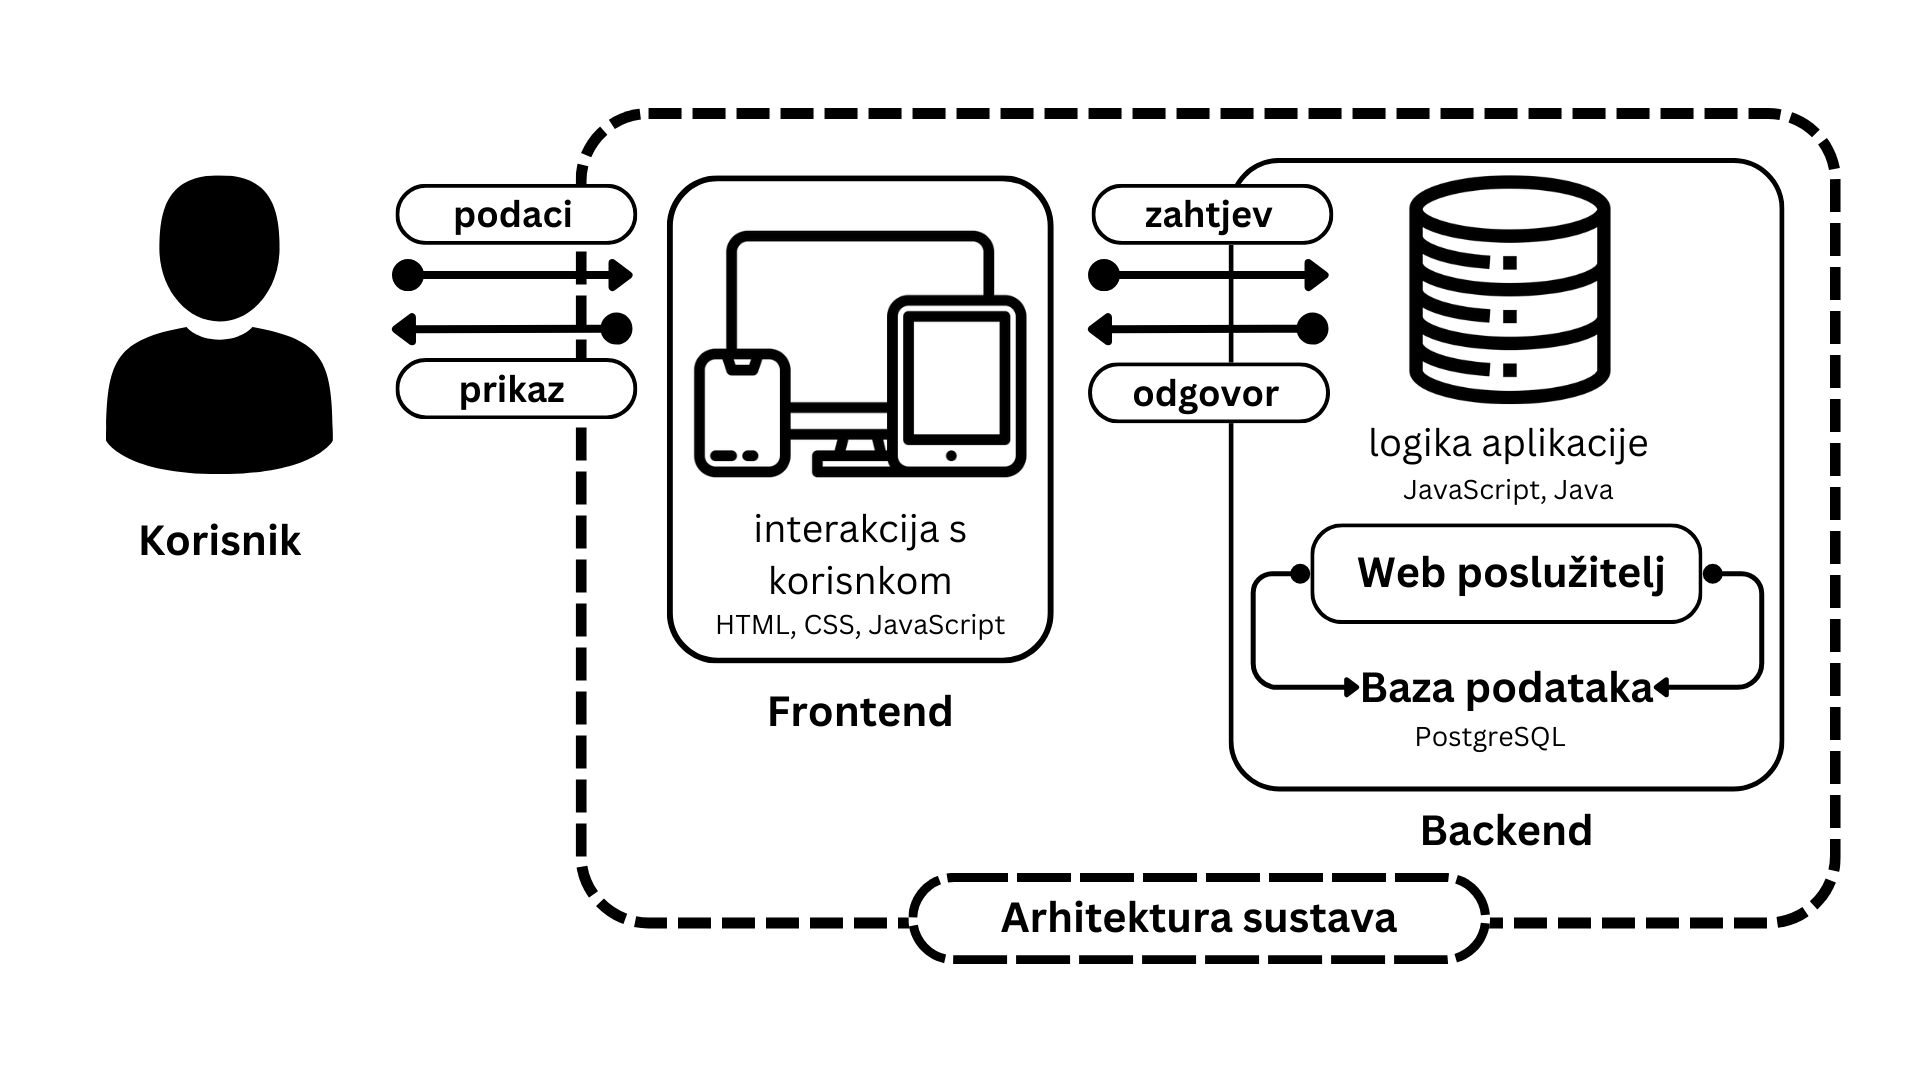
\includegraphics[scale=0.25]{slike/Arhitektura_sustava.png} %veličina slike u odnosu na originalnu datoteku i pozicija slike
	\centering
	\caption{Arhitektura sustava}
	\label{fig:Arhitektura}
\end{figure}


\section{Baza podataka}

\noindent Sustav je temeljen na uporabi relacijske baze podataka implementirane u PostgreSQL-u gdje su entiteti modelirani kao tablice koje posjeduju svoje jedinstveno ime i skup atributa.
Odabir relacijske baze podataka proizlazi iz potrebe za lakšim ostvarenjem naših potreba za upravljanjem podacima pri prijavljivanju oštećenja i njihovoj sanaciji
odnosno kako bismo što jednostavnije modelirali sustav prema stvarnom svijetu.
Ova baza podataka ključna je za sigurnost podataka i brz pristup, pohranu, umetanje, izmjenu te dohvat podataka koje sustav koristi za daljnju obradu.
Baza podataka ove aplikacija sadrži sljedeće entitete:
\begin{packed_item}
	\item \textit{Users}
	\item \textit{Reports}
	\item \textit{CityDept}
	\item \textit{Category}
	\item \textit{Problems}
	\item \textit{Photo}
\end{packed_item}



\subsection{Opis tablica}

\noindent \textbf{Users} je entitet koji sadrži sve bitne informacije o korisnicima i njihovim ulogama unutar aplikacije.
Sastoji se od atributa: user\_id, firstname, lastname, email, password, role i city\_dept\_id.
Povezan je vezom \textit{Many-to-One} s entitetom CityDept preko atributa city\_dept\_id i vezom \textit{One-to-Many} s entitetom Reports preko atributa user\_id.


\begin{longtblr}[
	label=none,
	entry=none
	]{
	width = \textwidth,
	colspec={|X[6,l]|X[6, l]|X[20, l]|},
	rowhead = 1,
	} %definicija širine tablice, širine stupaca, poravnanje i broja redaka naslova tablice
	\hline \SetCell[c=3]{c}{\textbf{Users}}                                                                           \\ \hline[3pt]
	\SetCell{LightGreen}user\_id       & INT     & jedinstveni identifikator korisnika                                \\ \hline
	firstname                          & VARCHAR & ime korisnika                                                      \\ \hline
	lastname                           & VARCHAR & prezime korisnika                                                  \\ \hline
	email                              & VARCHAR & e-mail adresa korisnika                                            \\ \hline
	password                           & VARCHAR & hash lozinke korisnika                                             \\ \hline
	role                               & VARCHAR & uloga korisnika                                                    \\ \hline
	\SetCell{LightBlue} city\_dept\_id & INT     & jedinstveni identifikator gradskog ureda (citydept.city\_dept\_id) \\ \hline
\end{longtblr}


\noindent\textbf{Reports} je entitet koji sadrži sve bitne informacije o prijavama oštećenja.
Sastoji se od atributa: report\_id, user\_id, title, description, address, report\_time, status, problem\_id, longitude, latitude i business\_id.
Povezan je vezom \textit{Many-to-One} s entitetom Problems preko atributa problem\_id, vezom \textit{Many-to-One} s entitetom Users preko atributa user\_id i vezom \textit{One-to-Many} s entitetom Photo preko atributa report\_id.
\begin{longtblr}[
	label=none,
	entry=none
	]{
	width = \textwidth,
	colspec={|X[6,l]|X[6, l]|X[20, l]|},
	rowhead = 1,
	} %definicija širine tablice, širine stupaca, poravnanje i broja redaka naslova tablice
	\hline \SetCell[c=3]{c}{\textbf{Reports}}                                                                \\ \hline[3pt]
	\SetCell{LightGreen}report\_id  & INT       & jedinstveni identifikator prijave                          \\ \hline
	\SetCell{LightBlue} user\_id    & INT       & jedinstveni identifikator korisnika (users.user\_id)       \\ \hline
	title                           & VARCHAR   & naziv prijave/oštećenja                                    \\ \hline
	description                     & TEXT      & opis oštećenja                                             \\ \hline
	address                         & VARCHAR   & adresa oštećenja                                           \\ \hline
	report\_time                    & TIMESTAMP & vrijeme podnošenja prijave                                 \\ \hline
	status                          & VARCHAR   & status prijave                                             \\ \hline
	longitude                       & DOUBLE    & geografska dužina lokacije oštećenja                       \\ \hline
	latitude                        & DOUBLE    & geografska širina lokacije oštećenja                       \\ \hline
	business\_id                    & UUID      & jedinstveni identifikator anonimne prijave                 \\ \hline
	\SetCell{LightBlue} problem\_id & INT       & jedinstveni identifikator oštećenja (problems.problem\_id) \\ \hline
\end{longtblr}

\noindent\textbf{CityDept} je entitet koji sadrži sve bitne informacije o gradskim uredima.
Sastoji se od atributa: city\_dept\_id, city\_dept\_name i category\_id.
Povezan je vezom \textit{One-to-Many} s entitetom Users preko atributa city\_dept\_id i vezom \textit{One-to-One} s entitetom Category preko atributa category\_id.
\begin{longtblr}[
	label=none,
	entry=none
	]{
	width = \textwidth,
	colspec={|X[6,l]|X[6, l]|X[20, l]|},
	rowhead = 1,
	} %definicija širine tablice, širine stupaca, poravnanje i broja redaka naslova tablice
	\hline \SetCell[c=3]{c}{\textbf{CityDept}}                                                                            \\ \hline[3pt]
	\SetCell{LightGreen}city\_dept\_id & INT     & jedinstveni identifikator gradskog ureda                               \\ \hline
	city\_dept\_name                   & VARCHAR & naziv gradskog ureda                                                   \\ \hline
	\SetCell{LightBlue} category\_id   & INT     & jedinstveni identifikator kategorije oštećenja (category.category\_id) \\ \hline
\end{longtblr}

\noindent\textbf{Category} je entitet koji sadrži sve bitne informacije o kategoriji oštećenja.
Sastoji se od atributa: category\_id i category\_name.
Povezan je vezom \textit{One-to-Many} s entitetom Problems preko atributa category\_id i vezom \textit{One-to-One} s entitetom CityDept preko atributa category\_id.
\begin{longtblr}[
	label=none,
	entry=none
	]{
	width = \textwidth,
	colspec={|X[6,l]|X[6, l]|X[20, l]|},
	rowhead = 1,
	} %definicija širine tablice, širine stupaca, poravnanje i broja redaka naslova tablice
	\hline \SetCell[c=3]{c}{\textbf{Category}}                                                  \\ \hline[3pt]
	\SetCell{LightGreen}category\_id & INT     & jedinstveni identifikator kategorije oštećenja \\ \hline
	category\_name                   & VARCHAR & naziv kategorije oštećenja                     \\ \hline
\end{longtblr}

\noindent\textbf{Problems} je entitet koji sadrži sve bitne informacije o prijavljenom oštećenju.
Sastoji se od atributa: problem\_id, longitude, latitude, status i category\_id.
Povezan je vezom \textit{One-to-Many} s entitetom Reports preko atributa problem\_id i vezom \textit{Many-to-One} s entitetom Category preko atributa category\_id.
\begin{longtblr}[
	label=none,
	entry=none
	]{
	width = \textwidth,
	colspec={|X[6,l]|X[6, l]|X[20, l]|},
	rowhead = 1,
	} %definicija širine tablice, širine stupaca, poravnanje i broja redaka naslova tablice
	\hline \SetCell[c=3]{c}{\textbf{Problems}}                                                                           \\ \hline[3pt]
	\SetCell{LightGreen}problem\_id  & INT     & jedinstveni identifikator oštećenja                                     \\ \hline
	longitude                        & DOUBLE  & geografska dužina lokacije oštećenja                                    \\ \hline
	latitude                         & DOUBLE  & geografska širina lokacije oštećenja                                    \\ \hline
	status                           & VARCHAR & status oštećenja                                                        \\ \hline
	\SetCell{LightBlue} category\_id & INT     & jedinstveni identifikator kategorije oštećenja  (category.category\_id) \\ \hline
\end{longtblr}


\noindent\textbf{Photo} je entitet koji sadrži sve bitne informacije vezane za sliku oštećenja.
Sastoji se od atributa: photo\_id, photo\_data i report\_id.
Povezan je vezom \textit{Many-to-One} s entitetom Reports preko atributa report\_id.

\begin{longtblr}[
	label=none,
	entry=none
	]{
	width = \textwidth,
	colspec={|X[6,l]|X[6, l]|X[20, l]|},
	rowhead = 1,
	} %definicija širine tablice, širine stupaca, poravnanje i broja redaka naslova tablice
	\hline \SetCell[c=3]{c}{\textbf{Photo}}                                                       \\ \hline[3pt]
	\SetCell{LightGreen}photo\_id & INT   & jedinstveni identifikator slike (photo.photo\_id)     \\ \hline
	photo\_data                   & BYTEA & slika oštećenja                                       \\ \hline
	\SetCell{LightBlue}report\_id & INT   & jedinstveni identifikator prijave (report.report\_id) \\ \hline
\end{longtblr}


\subsection{Dijagram baze podataka}

\begin{figure}[H]
	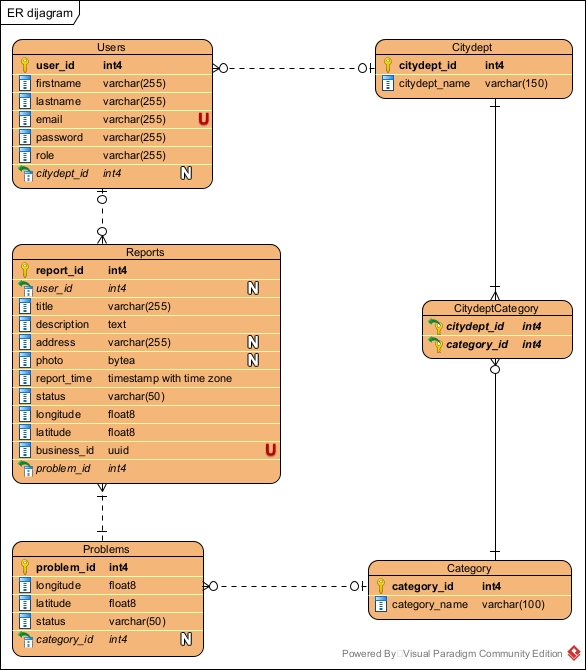
\includegraphics[scale=0.75]{slike/ERD-model} %veličina slike u odnosu na originalnu datoteku i pozicija slike
	\centering
	\caption{E-R dijagram baze podataka}
	\label{fig:ERdijagramBazePodataka}
\end{figure}

\eject


\section{Dijagram razreda}

Na slikama 4.3, 4.4, 4.5 i 4.6 prikazani su razredi koji pripadaju \textit{backend} dijelu
s arhitekturom podijeljenom na kontrolere, repozitorije i servise te uključuje DTO
(Data Transfer Object) i modele. \newline

Na slikama 4.3 i 4.4 prikazani su razredi koji nasljeđuju Controller razred. Metode implementirane u tim razredima
upravljaju i rukuju DTO-ima koji su dohvaćeni pomoću metoda implementiranih u Model razredima. Omogućuju
logiku interakcije i promjene. Kontroler AuthenticationController omogućuje registraciju i prijavu korisnika.
Kontroler ReportController omogućuje interakcije s prijavom oštećenja, dok kontroler ProblemController omogućuje
interakcije s objedinjenim problemima oštećenja s istom temom i lokacijom. Kontroler UserController omogućuje
interakcije i promjene povezane s registriranim korisnicima. Kontroler CityDeptController omogućuje
interakcije i promjene povezane s gradskim uredima. Kontroler PhotoController omogućuje interakciju i promjene
vezane za slike oštećenja. Kontroler CategoryController omogućuje interakciju i promjene vezane za
kategorije oštećenja. Kontroler ExceptionController omogućuje interakcije vezane za iznimke.

\begin{figure}[H]
	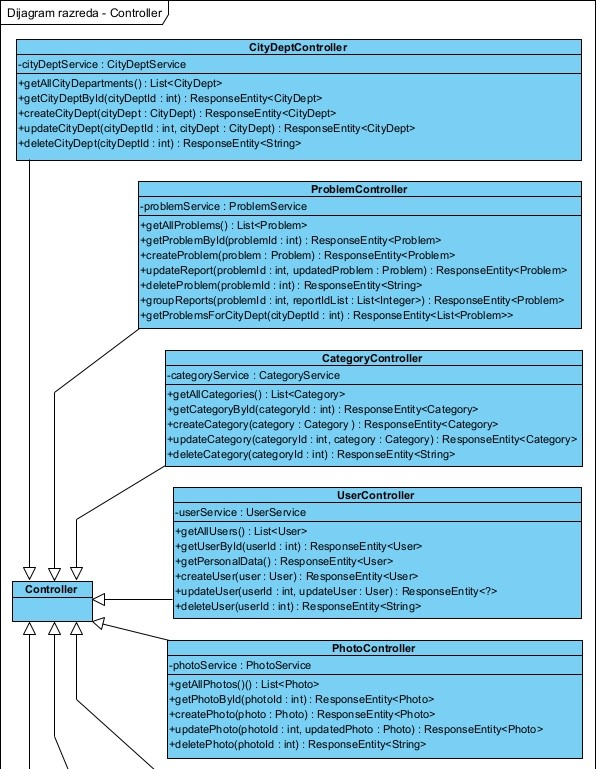
\includegraphics[scale=1.0]{slike/DR-controller1} %veličina slike u odnosu na originalnu datoteku i pozicija slike
	\centering
	\caption{Dijagram razreda - dio Controllers - prvi dio}
	\label{fig:DijagramRazredaControllers}
\end{figure}

\begin{figure}[H]
	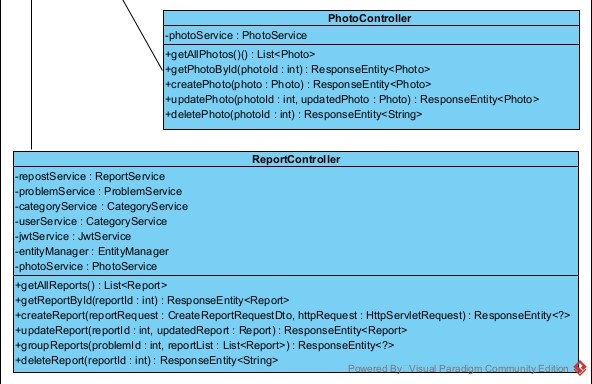
\includegraphics[scale=1.0]{slike/DR-controller2} %veličina slike u odnosu na originalnu datoteku i pozicija slike
	\centering
	\caption{Dijagram razreda - dio Controllers - drugi dio}
	\label{fig:DijagramRazredaControllers}
\end{figure}

Na slici 4.4 prikazani su razredi koji pripadaju DTO. Data Transfer Objects (DTO) omogućavaju
razmjenu podataka između procesa i slojeva. RegisterRequestDto služi za registraciju korisnika.
LoginRequestDto služi za prijavu korisnika. AuthenticationResponseDto sastoji se od jwt tokena koji se vraća
kada se korisnik registrira ili ulogira. ReportRequestDto služi za kreiranje podataka o prijavi
oštećenja i problema.

\begin{figure}[H]
	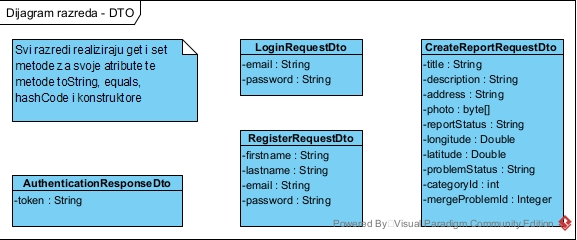
\includegraphics[scale=0.60]{slike/DR-DTO.jpg} %veličina slike u odnosu na originalnu datoteku i pozicija slike
	\centering
	\caption{Dijagram razreda - dio DTO}
	\label{fig:DijagramRazredaDTO}
\end{figure}

Na slici 4.5 prikazi su razredi koji pripadaju Model razredima. Oni preslikavaju strukturu baze podataka
u aplikaciji. Komuniciraju s bazom podataka te vraćaju podatke iz nje. Razred User predstavlja registriranog
korisnika koji je unio nužne podatke u sustav. Razred Report predstavlja prijavu oštećenja za koju je korisnik
unio potrebne i opcionalne podatke. Razred Problem predstavlja prijavu problema koja predstavlja jednu ili više
prijava oštećenja objedinjene u prijavu problema sa zajedničkom temom i lokacijom. Razred Category predstavlja
kategoriju oštećenja koju korisnik može odabrati za prijavljeno oštećenje, odnosno koju gradski ured može dobiti
na upravljanje oštećenjima. Razred CityDept predstavlja gradski ured koji upravlja jednom kategorijom oštećenja
koju im je administrator dodijelio. Enumeracija Role predstavlja ulogu koju registrirani korisnik ima. Razred
Photo predstavlja fotografiju oštećenja koju je korisnik dodao prilikom prijave oštećenja.

\begin{figure}[H]
	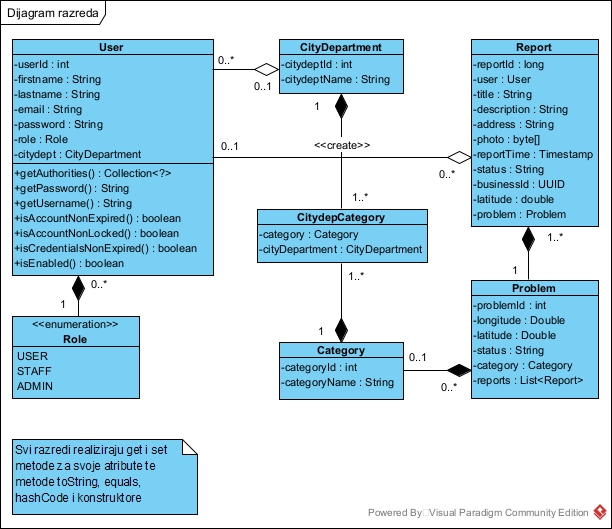
\includegraphics[scale=0.60]{slike/DR-model.jpg} %veličina slike u odnosu na originalnu datoteku i pozicija slike
	\centering
	\caption{Dijagram razreda - dio Model}
	\label{fig:DijagramRazredaModel}
\end{figure}


\textbf{\textit{dio 2. revizije}}\\

\textit{Prilikom druge predaje projekta dijagram razreda i opisi moraju odgovarati stvarnom stanju implementacije}



\eject

\section{Dijagram stanja}


\textbf{\textit{dio 2. revizije}}\\

\textit{Potrebno je priložiti dijagram stanja i opisati ga. Dovoljan je jedan dijagram stanja koji prikazuje \textbf{značajan dio funkcionalnosti} sustava. Na primjer, stanja korisničkog sučelja i tijek korištenja neke ključne funkcionalnosti jesu značajan dio sustava, a registracija i prijava nisu. }

Dijagram stanja, poznat i kao state machine diagram, je ponašajni UML-dijagram koji se koristi za jasno definiranje mogućih stanja objekta, identifikaciju prijelaza između tih stanja i prikaz ponašanja sustava u različitim situacijama.
Na slici 4.6 prikazan je dijagram stanja za prijavljenog korisnika. Nakon prijave, korisniku se prikazuje početna stranica s kartografskim prikazom na kojem su crvenim markerima označene već podnesene prijave određenih šteta na javnim površinama.
Odabirom nekog crvenog markera, korisniku se prikazuju informacije o konkretnoj podnesenoj prijavi. Sličnu funkcionalnost korisnik ostvaruje upisom identifikacijskog broja prijave u zaglavlju čime mu se prikazuju informacije, odnosno status neke od vlastitih podnesenih prijava. Osim pregleda statusa podnesenih šteta, pomoću zaglavlja aplikacije korisnik može pristupiti svom korisničkom računu, pregledati statistiku svih do tog trenutka podnesenih prijava te pristupiti podnošenju nove prijave. Prilikom podnošenja nove prijave, osim unošenja podataka o nastaloj šteti, korisnik može odabrati sliku s vlastitog uređaja i odabrati lokaciju štete na karti. Također, pomoću padajućeg izbornika u zaglavlju, korisnik se može odjaviti iz sustava. S obzirom na to da je zaglavlje zastupljeno na svim stranicama aplikacije, korisnik svim navedenim opcijama vezanim uz zaglavlje može pristupiti neovisno o tome gdje se nalazi unutar aplikacije. Pristupom u vlastiti korisnički račun, omogućen je pregled i uređivanje osobnih podataka, pregled podnesenih prijava korisnika kao i brisanje računa. Ako korisnik prilikom pregleda informacija vlastitih podnesenih prijava, odabere jednu od njih, pristupa informacijama o svim bliskim prijavama odabrane prijave.
\begin{figure}[H]
	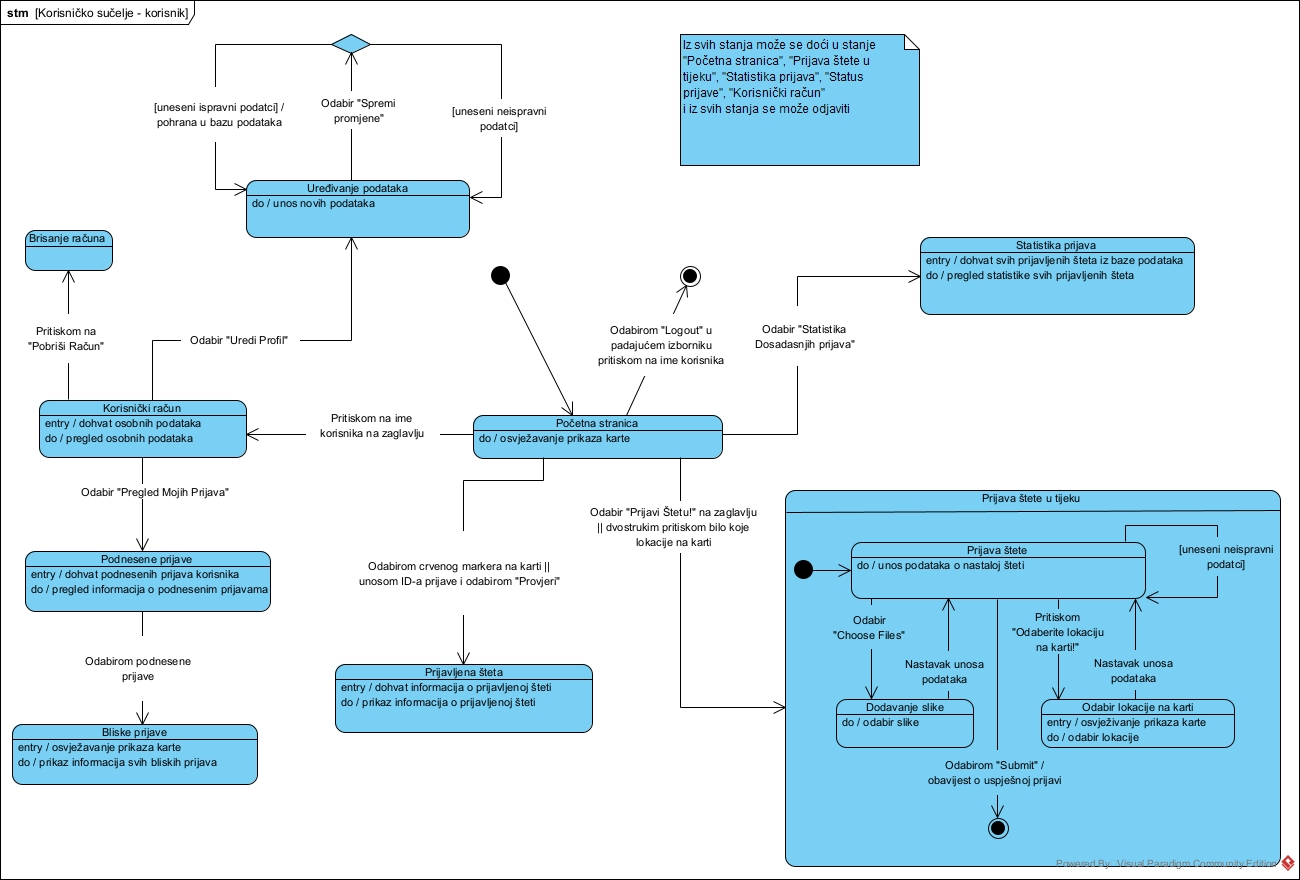
\includegraphics[scale=0.35]{slike/DS.jpg} %veličina slike u odnosu na originalnu datoteku i pozicija slike
	\centering
	\caption{Dijagram stanja}
	\label{fig:DijagramStanja}
\end{figure}

\eject

\section{Dijagram aktivnosti}

\textbf{\textit{dio 2. revizije}}\\

\textit{Potrebno je priložiti dijagram aktivnosti s pripadajućim opisom. Dijagram aktivnosti treba prikazivati značajan dio sustava.}

UML-dijagrami aktivnosti (activity diagrams) predstavljaju ponašajne dijagrame koji se koriste za modeliranje i grafički prikaz dinamičkog ponašanja sustava.
Ovi dijagrami vizualiziraju izvođenje aktivnosti kroz niz akcija koje kontroliraju tokove i objekte, s posebnim naglaskom na slijed i uvjete toka.
Dijagrami aktivnosti omogućuju jasno predstavljanje redoslijeda izvođenja aktivnosti, čime olakšavaju razumijevanje dinamike sustava.
Na dijagramu aktivnosti sa slike 4.7 prikazan je proces podnošenja nove prijave štete neprijavljenog korisnika.
Korisnik se prijavi u sustav, zatim odabirom lokacije na karti ili odabirom "Prijavi Štetu!" na zaglavlju, unosi podatke o nastaloj šteti u prikazanoj formi za prijavu.
Ako su podaci neispravno uneseni, korisniku se omogućuje ponovni upis podataka, a ako su podaci ispravni, spremaju se u bazu podataka te se korisniku prikazuje potvrda o uspješno podnesenoj prijavi zajedno s identifikacijskim brojem prijave, kako bi mogao provjeriti status podnesene prijave. Korisnik je pri završetku procesa pozicioniran ponovno na početnu stranicu.

\begin{figure}[H]
	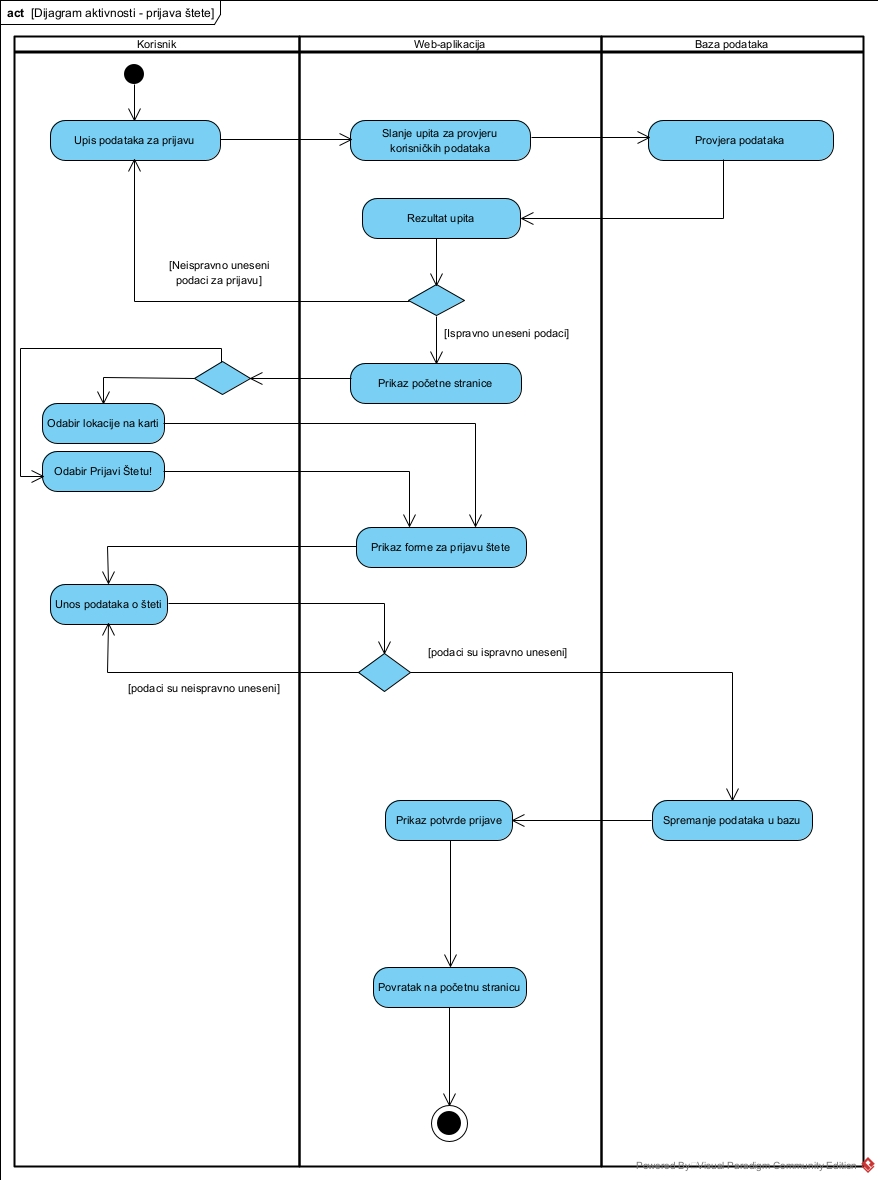
\includegraphics[scale=0.5]{slike/DA.jpg} %veličina slike u odnosu na originalnu datoteku i pozicija slike
	\centering
	\caption{Dijagram aktivnosti}
	\label{fig:DijagramAktivnosti}
\end{figure}

\eject
\section{Dijagram komponenti}

\textbf{\textit{dio 2. revizije}}\\

\textit{Potrebno je priložiti dijagram komponenti s pripadajućim opisom. Dijagram komponenti treba prikazivati strukturu cijele aplikacije.}

Dijagram komponenti prikazan je na slici 4.9 te služi za vizualizaciju organizacije i međuovisnosti implementacijskih
komponenata (interna struktura) te odnos programske potpore prema okolini. Sustavu se pristupa preko web preglednika pomoću sučelja HTTP\_REQUEST
na kojem se poslužuju datoteke koje pripadaju \textit{frontend} dijelu aplikacije. \textit{Frontend} dio nazvan React Frontend
sastoji se od komponenti React View, React router, ReactJS, Index.js, Content.js, React leaflet te sučelja REST\_API i MAP\_API.
React View komponenta komunicira s \textit{backendom} preko sučelja REST\_API i razmjenjuje podatke s \textit{backendom} u
JSON formatu, te ovisno o korisnikovim akcijama osvježava prikaz na stranici. Komponenta React router na temelju URL-a
odlučuje koja će se stranica prikazati, odnosno datoteka dohvatiti. Komponenta ReactJS je centralna biblioteka za React
preko koje se dobivaju gotove komponente za prikaz. Komponenta Index.js služi kao početna komponenta unutar koje se nalazi
organizirana hijerarhija ostalih elemenata za prikaz. Jedan od njih je komponenta Content.js koja služi za ostvarivanje
prikaza karte. Integraciju interaktivnih karata i manipulaciju geografskih podataka s React aplikacijama omogućava biblioteka
React leaflet prikazana komponentom React leaflet. Sučelje MAP\_API koristi se za razmjenu podataka s vanjskom komponentom
Openstreetmaps. \textit{Backend} dio nazvan Spring Boot backend sastoji se od komponenti RestController, JPA repository,
Controller, Service, Model, Repository, DTO te sučelja REST\_API, PSQL, JPA i GEOCODING\_API. Komponenta RestController komunicira
s \textit{frontendom} preko sučelja REST\_API i razmjenjuje podatke u JSON formatu. Komponenta JPA repository predstavlja
dio Spring Data JPA koji omogućava jednostavan pristup podacima u bazi podataka koristeći PSQL sučelje za komuniciranje i
razmjenu podataka s vanjskom komponentnom PostgreSQL baza podataka te sučelja JPA za komunikaciju s komponentnom Repository.
Komponenta Controller prima zahtjeve, provjerava ih te šalje odgovore na dobivene zahtjeve prema klijentskoj strani. Komponenta
Service prima zahtjeve od Controller, obrađuje ih i prosljeđuje komponentni Repository. Komponenta Model predstavlja entitete
koji se pohranjuju u bazi podataka. Komponenta DTO predstavlja oblik objekta koji se koristi za prijenos podataka između
dijelova aplikacije. Sučelje GEOCODING\_API komunicira s vanjskom komponentom Geocoding koja služi za pretvaranje adrese
u geografske koordinate i obrnuto.


\begin{figure}[H]
	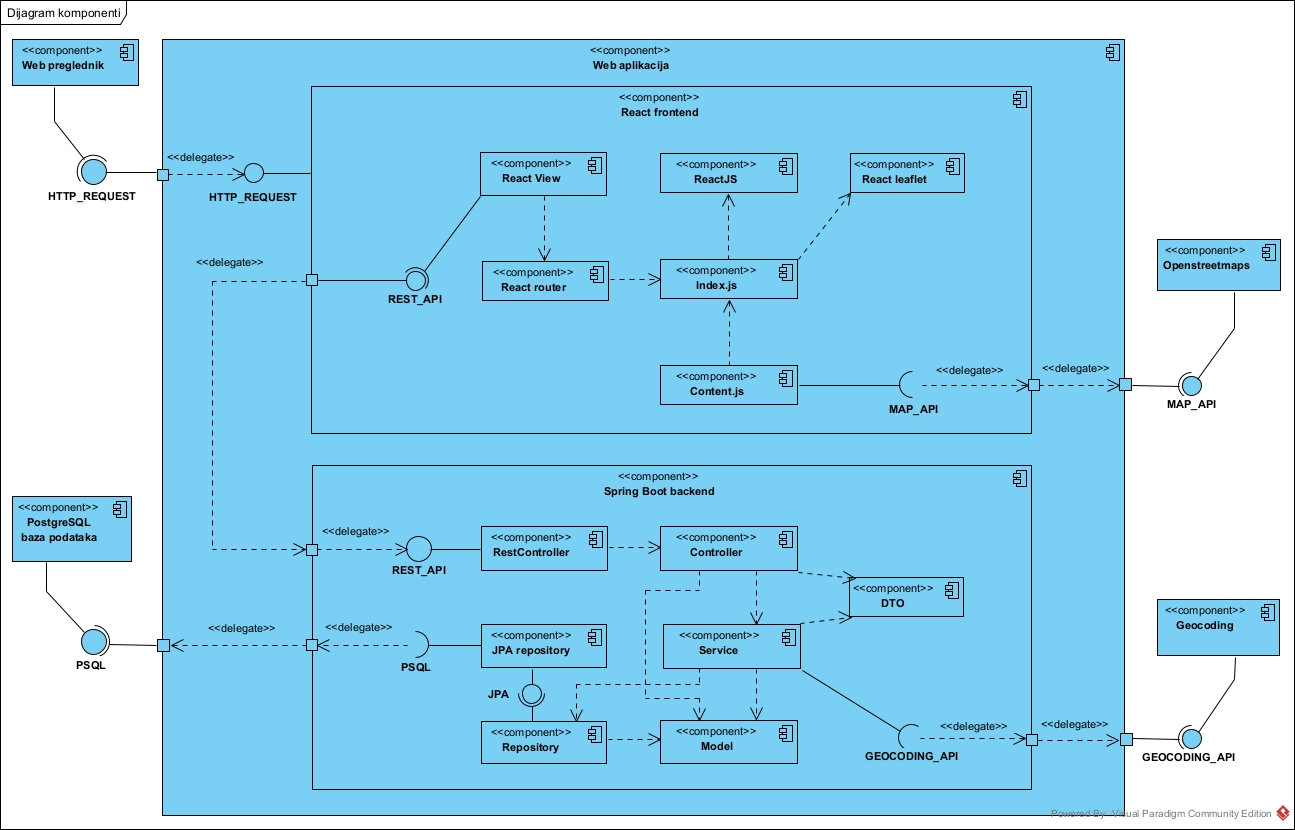
\includegraphics[scale=0.35]{slike/DK.jpg} %veličina slike u odnosu na originalnu datoteku i pozicija slike
	\centering
	\caption{Dijagram komponenti}
	\label{fig:DijagramKomponenti}
\end{figure}